% CHAPTER 1
\chapter{Introduction}
\label{chap:introduction}


% 1.1 HYDROGENIC ATOMS

Accurately describing the behaviour of electrons is fundamental to understanding atomic structure, chemical bonding and the properties of materials. However, most atomic and molecular systems cannot be solved analytically, making numerical approximations essential in computational physics and chemistry. Hydrogen and hydrogenic ions provide an ideal starting point for investigating the reliability of these methods, as their exact non-relativistic energies and wavefunctions are known. This allows the accuracy of an approximation to be measured directly rather than inferred from numerical convergence alone. Importantly, reproducing an accurate energy does not necessarily guarantee an equally accurate wavefunction, while increasing the complexity of an approximation can introduce additional numerical difficulties. These considerations highlight the importance of constructing approximations that balance physical accuracy, numerical reliability and computational efficiency. Such methods underpin modern computational chemistry, with applications ranging from pharmaceutical research, where quantum-mechanical calculations help investigate drug–receptor interactions and chemical reactivity \cite{heifetz2020}, to astrochemistry, where predicted molecular properties and spectra help identify complex and potentially prebiotic molecules in interstellar environments \cite{barone2015}.
\section{Hydrogenic Atoms}

Hydrogenic atoms contain a single electron bound to a
nucleus of charge $+Ze$, where $Z$ is the atomic number.
Hydrogen ($Z=1$) is the simplest example, but the same
model also describes one-electron ions such as
$\mathrm{He}^{+}$, $\mathrm{Li}^{2+}$ and
$\mathrm{Mn}^{24+}$. Unlike multi-electron atoms, hydrogenic systems have no electron--electron interactions. Their non-relativistic Schrödinger equation can therefore be solved analytically, providing exact wavefunctions and energies against which numerical approximations can be tested.

In atomic units, assuming an infinitely massive point
nucleus, the Hamiltonian is
\begin{equation}
    \hat{H}=-\frac{1}{2}\nabla^2-\frac{Z}{r},
    \label{eq:intro_hamiltonian}
\end{equation}
where $r$ is the electron--nucleus separation.
The exact ground-state energy and normalised
$1s$ wavefunction are
\begin{equation}
    E_{1s}=-\frac{Z^2}{2},
    \qquad
    \psi_{1s}(r)
    =\sqrt{\frac{Z^3}{\pi}}e^{-Zr}.
    \label{eq:intro_hydrogenic}
\end{equation}

As $Z$ increases, the electron becomes more tightly
bound and its wavefunction becomes more concentrated
near the nucleus. The ground-state energy scales as
$Z^2$, while the characteristic radial length scale
decreases as $1/Z$.

\begin{figure}[htbp]
    \centering
    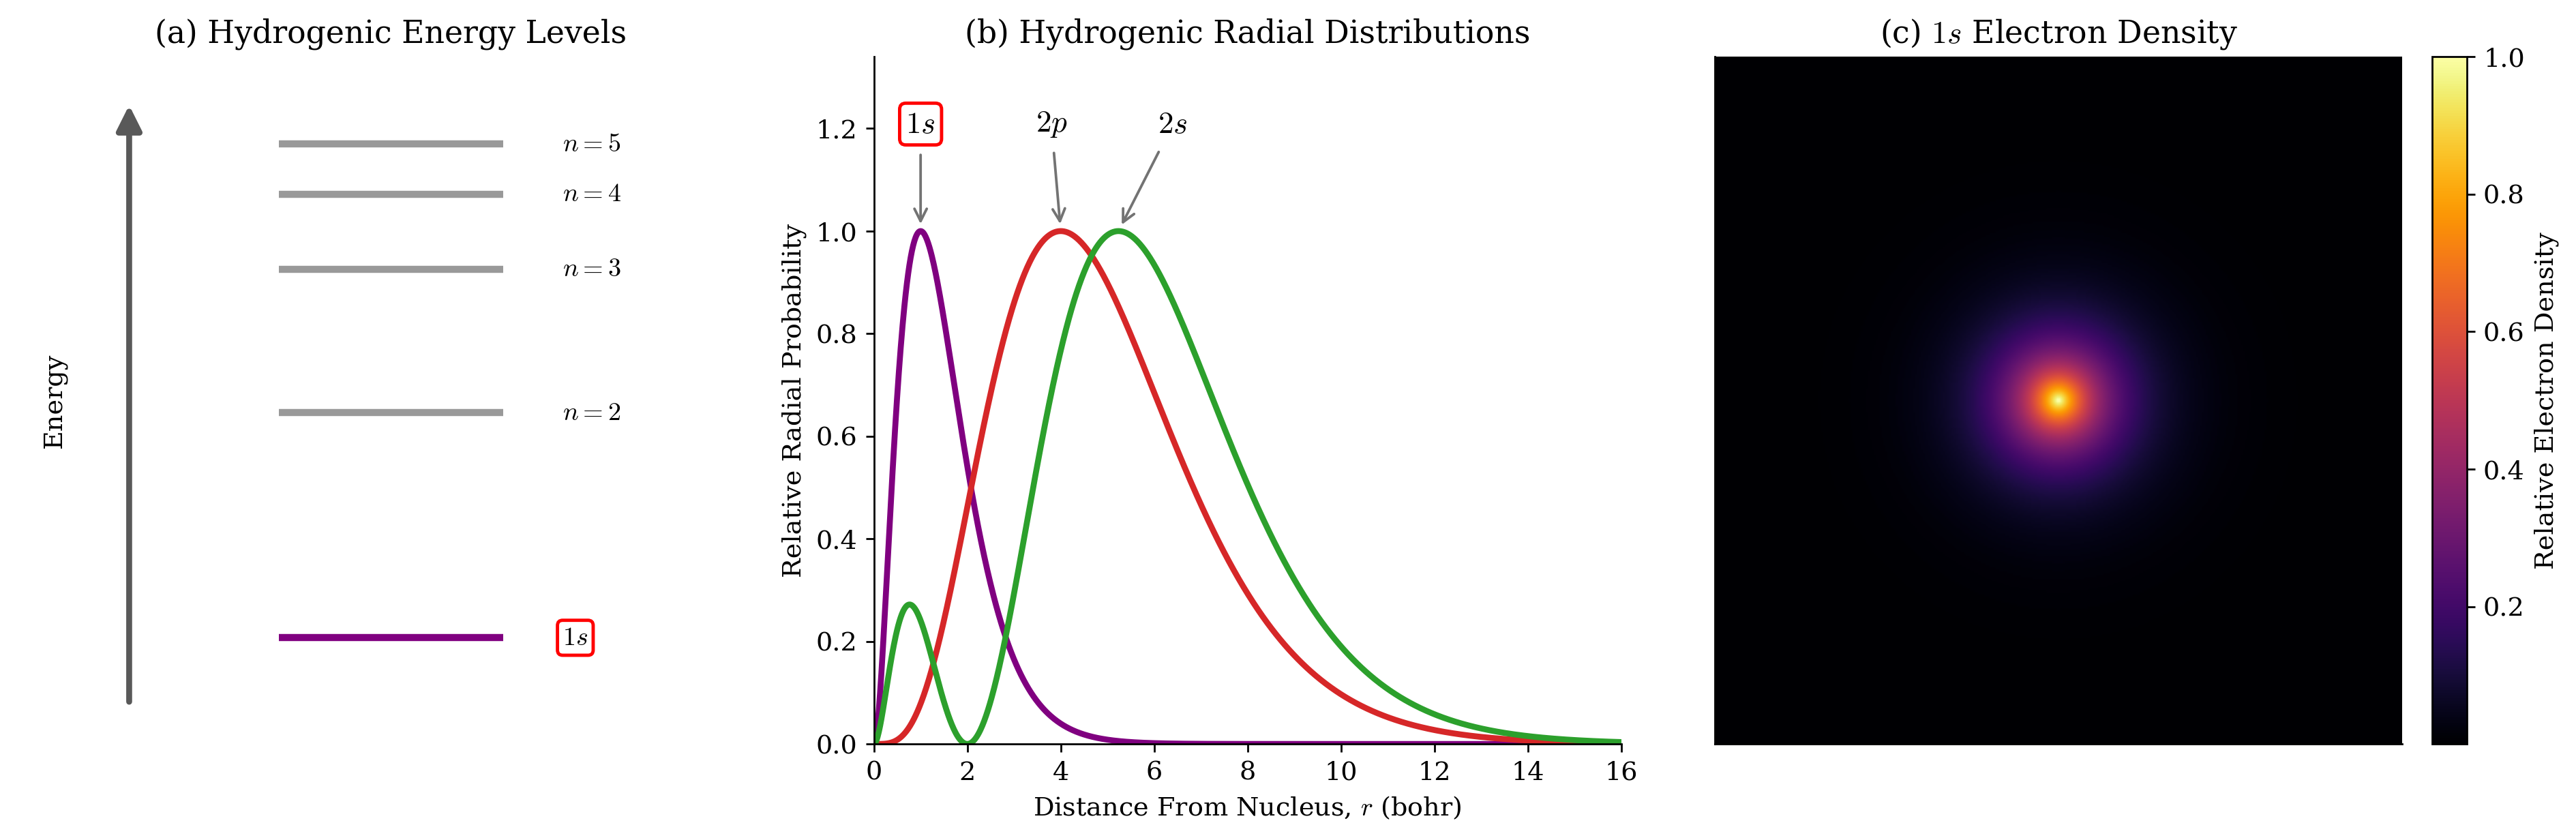
\includegraphics[width=\linewidth]
    {Figures/Chapter1_Panel.png}
    \caption{Overview of the hydrogenic atom:
    (a) discrete electronic energy levels,
    (b) radial probability distributions for the
    $1s$, $2s$ and $2p$ orbitals, and
    (c) the spatial electron density of the
    $1s$ orbital. The focus here is on the
    ground state, for which exact results
    provide a reference for numerical calculations.}
    \label{fig:hydrogenic_overview}
\end{figure}

Hydrogenic systems are therefore useful for examining
the accuracy, convergence and numerical stability of
approximate quantum-mechanical methods. Since the exact
solution is known, errors can be measured directly
without uncertainty in the reference values.



% 1.2 GAUSSIAN BASIS SETS

\newpage
\section{Gaussian Basis Sets}

Although the hydrogenic Schrödinger equation has an
exact solution, most atomic and molecular systems
cannot be solved analytically. Numerical
electronic-structure methods therefore approximate
wavefunctions using finite combinations of simpler
functions, known as basis functions.

One common choice is the Gaussian function, introduced
into electronic-structure calculations by Boys
\cite{Boys1950}. A spherical Gaussian has the form
\begin{equation}
    \phi_i(r)=A_i e^{-\lambda_i r^2},
    \label{eq:intro_gaussian}
\end{equation}
where $\lambda_i>0$ determines its spatial width
and $A_i$ is a normalisation constant. Small exponents
give broad functions extending farther from the nucleus,
while large exponents give narrow functions concentrated
near it.

The hydrogenic ground-state wavefunction can be
approximated by a linear combination of $N$ Gaussians,
\begin{equation}
    \psi_{\mathrm G}(r)
    =\sum_{i=1}^{N}c_i\phi_i(r),
    \label{eq:intro_expansion}
\end{equation}
where the coefficients $c_i$ determine the contribution
of each function. These coefficients are found by
minimising the energy expectation value, leading to
a generalised eigenvalue problem. Its eigenvalues
give approximate energies, while its eigenvectors
determine the corresponding wavefunctions.

The main computational advantage of Gaussian functions
is that their products and many of the required
integrals can be evaluated analytically. This makes
them useful for constructing the Hamiltonian and
overlap matrices in electronic-structure calculations
\cite{Boys1950}. Gaussian basis sets are widely used
in quantum chemistry, including in contracted and
correlation-consistent basis sets
\cite{Dunning1989,Raffenetti}.

The choice of Gaussian exponents determines the range
of distances that the basis can represent. Here, the
exponents follow a geometric sequence,
\begin{equation}
    \lambda_i=\alpha\beta^{i-1},
    \qquad i=1,\ldots,N,
    \label{eq:intro_even_tempered}
\end{equation}
where $\alpha>0$ sets the smallest exponent,
$\beta>1$ controls the spacing between successive
exponents, and $N$ is the number of functions.

This is known as an \textit{even-tempered Gaussian
basis}. Each exponent is $\beta$ times the previous
one, giving equal spacing on a logarithmic scale.
Changing $N$, $\alpha$ and $\beta$ therefore allows
the number and distribution of functions to be
adjusted systematically.
Even-tempered bases and Gaussian exponent optimisation
have been studied by Feller and Ruedenberg
\cite{FellerRuedenberg1979}, Bardo and Ruedenberg
\cite{BaR}, and Wilson \cite{Wilson}.

\newpage

% 1.3 ACCURACY AND LIMITATIONS

\section{Accuracy and Limitations of Gaussian Expansions}

Despite their computational advantages, Gaussian
functions do not have the same radial behaviour
as exact hydrogenic wavefunctions. The exact
$1s$ wavefunction decreases as $e^{-Zr}$,
whereas an individual Gaussian decreases as
$e^{-\lambda r^2}$. A finite sum of Gaussians
can approximate the exact wavefunction closely
over a range of distances, but cannot reproduce
it exactly everywhere.

An important difference occurs at the nucleus.
The exact hydrogenic wavefunction satisfies
the electron--nucleus cusp condition:
\begin{equation}
    \left.
    \frac{\mathrm d\psi_{1s}}{\mathrm dr}
    \right|_{r=0}
    =-Z\psi_{1s}(0),
    \label{eq:intro_cusp}
\end{equation}
whereas the radial derivative of any finite
sum of centred spherical Gaussians is zero
at $r=0$. This limitation is related to the
Coulomb interaction near the nucleus
\cite{Kato,Kutzelnigg1994}.

This leads to an important distinction between
energy and wavefunction accuracy. The variational
method gives an upper bound to the exact
ground-state energy, but a small energy error
does not mean that every feature of the
wavefunction is equally accurate. In particular,
the behaviour near the nucleus may still differ
noticeably from the exact solution.

Adding more Gaussians generally makes the basis
more flexible, although the improvement depends
on the chosen exponents. Functions with very
similar widths can become nearly linearly
dependent, making the overlap matrix poorly
conditioned and the numerical solution less
reliable \cite{Lehtola2019}.
A useful Gaussian basis therefore cannot be
judged by its size alone. Energy accuracy,
wavefunction accuracy and numerical conditioning
must all be considered.



% 1.4 MOTIVATION AND SCOPE

\section{Motivation and Scope}

Gaussian basis sets are widely used in computational
chemistry, particularly in electronic-structure
methods such as Hartree--Fock theory and density
functional theory \cite{Atkins}. These methods approximate
the electronic states of atoms and molecules,
allowing properties such as molecular energies,
charge distributions and chemical bonding to
be investigated. Such calculations contribute
to materials modelling, the interpretation of
electronic spectra and pharmaceutical research,
where understanding molecular stability,
reactivity and intermolecular interactions
is important. However, the accuracy of these
predictions depends partly on the number
and choice of basis functions. Too few functions,
or poorly chosen exponents, may give inaccurate
energies and electron distributions, while adding
more functions increases computational cost and
can introduce numerical instability. Choosing a
suitable basis therefore involves balancing
accuracy, flexibility and numerical reliability.

The hydrogenic ground state provides a useful
way to examine this problem because its exact
energy and wavefunction are known. Errors in the
Gaussian approximation can therefore be measured
directly, rather than relying only on whether
a calculation appears to have converged. This raises the 
central question:

\emph{How many Gaussian functions are needed
to reproduce a hydrogenic ground state to
a chosen accuracy while maintaining
numerical reliability?}

The first step is to compare the approximate
hydrogen energy, wavefunction and radial
probability distribution with their exact
values. Accuracy is then examined as the
number of Gaussians and the exponent parameters
$\alpha$ and $\beta$ are varied. The overlap
condition number provides a measure of numerical
reliability, while a parameter search identifies
the smallest tested bases meeting selected
energy-error targets. Comparing energy and
wavefunction errors also shows whether an
accurate energy is accompanied by an equally
accurate electron distribution.

A further question is whether a basis chosen
for hydrogen remains suitable for one-electron
ions with larger nuclear charges. As $Z$
increases, the electron distribution becomes
more concentrated near the nucleus, so the
original hydrogen exponents may no longer
cover the required range of distances.
To test this, fixed hydrogen exponents
are compared with those scaled by
\begin{equation}
    \lambda_i(Z)=Z^2\lambda_i(1),
    \label{eq:intro_scaling}
\end{equation}
which adjusts the Gaussian widths to match
the hydrogenic length scale. The comparison
covers $1\leq Z\leq25$, including
$\mathrm{Mn}^{24+}$, and considers both energy
accuracy and radial probability distributions.

The aim is not simply to obtain an accurate
ground-state energy, but to understand why
some Gaussian bases perform better than
others, how numerical reliability limits
their usefulness, and how the basis must
be adapted to the physical length scale
of the system. These questions are relevant
to basis-set selection in computational
chemistry, although the conclusions from
a one-electron model do not directly account
for the additional complexity of
many-electron systems.

All calculations use the non-relativistic,
fixed-nucleus, one-electron Hamiltonian
with spherical Gaussians centred on the
nucleus. Only ground states are considered.
Electron--electron interactions, molecular
geometry and relativistic effects are
outside the scope of this investigation.

Chapter~2 develops the theoretical framework,
Chapter~3 explains the numerical methods,
and Chapter~4 presents and discusses the
results. Chapter~5 summarises the main
findings and limitations.
